\section{Background}

\begin{figure}[t]
    \centering
    \begin{subfigure}[b]{0.46\columnwidth}
        \centering
        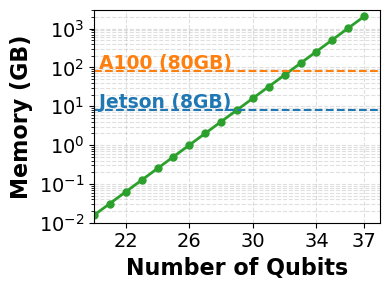
\includegraphics[width=\linewidth]{Figures/fig_motivation_a.png}
        \caption{Memory growth.}
        \label{intro_motivation_a}
    \end{subfigure}\hfill
    \begin{subfigure}[b]{0.50\columnwidth}
        \centering
        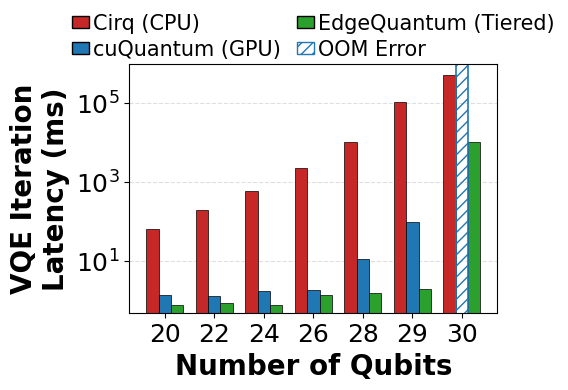
\includegraphics[width=\linewidth]{Figures/fig_motivation_b.png}
        \caption{VQE latency.}
        \label{intro_motivation_b}
    \end{subfigure}
    \caption{Memory wall and per-iteration VQE latency on resource-constrained edge devices.}
    \label{intro_motivation}
\end{figure}

\subsection{GPU-Accelerated Quantum Circuit Simulation}\label{back1}
Quantum circuit simulation involves trade-offs between scalability and computational complexity~\cite{qsim, svsim, suzuki2021qulacs, villalonga2019flexible}. Tensor network contraction reduces memory usage, but its computational cost grows exponentially for highly entangled circuits~\cite{gray2018quimb, lykov2022tensor, pan2022simulation}. In contrast, full state vector simulation explicitly maintains every probability amplitude, providing exact results regardless of circuit depth or entanglement structure~\cite{guerreschi2020intel, de2007massively, qsim, suzuki2021qulacs}. To process these vectors, simulators like \textit{cuStateVec}~\cite{bayraktar2023cuquantum} and \textit{Qiskit Aer}~\cite{qiskit} rely on GPU acceleration. They allocate the state vector in VRAM and process the circuit layer by layer, where CUDA kernels apply quantum gates in parallel, and data remains on-device, avoiding intermediate transfers.

\noindent\textbf{Memory Wall. }GPU-accelerated full state vector simulation is fundamentally limited by memory capacity. Memory footprint grows exponentially with the number of qubits at a complexity of $\mathcal{O}(2^n)$. Since each complex amplitude requires 8 bytes in single precision, a 30-qubit circuit demands 8GB, exhausting the 8GB limit of edge devices such as the NVIDIA Jetson Orin Nano. Scaling further, a 34-qubit circuit requires 128GB, and a 39-qubit circuit demands 4TB, far exceeding edge memory capacities. As shown in Figure~\ref{intro_motivation_a}, this exponential growth defines the memory wall on edge devices, while server-grade discrete GPUs such as the NVIDIA A100 sustain in-memory execution up to 80GB of dedicated VRAM. The wall is further amplified by the unified memory architecture: the 8GB physical DRAM is shared by the OS, CPU, and GPU, leaving insufficient headroom for kernel workspaces and runtime allocations once the state vector approaches the limit. 

\noindent\textbf{Per-iteration VQE Latency. }As shown in Figure~\ref{intro_motivation_b}, this memory wall manifests as the qubit count grows on edge devices. CPU-only execution (\textit{Cirq}) avoids GPU workspace overhead but pays orders-of-magnitude compute cost, requiring over 100 seconds (109,168ms) for a single 29-qubit VQE iteration. GPU-accelerated execution (\textit{cuQuantum}) fails to simulate 29 qubits, immediately crashing with an Out-of-Memory (OOM) error due to physical memory capacity constraints. To address this, out-of-core memory management is required. Existing frameworks~\cite{zhang2025bmqsim, wu2019full, li2021sv, park2022snuqs} employ data compression and tiered memory pipelines to mitigate memory limits. However, these approaches are optimized for server-grade GPUs with discrete PCIe topologies and abundant host resources. Adapting them to edge environments requires falling back to blocking I/O on external NVMe storage. Their pipelines assume host-driven DMA paths that are absent on UMA SoCs, stalling GPU computation and incurring severe I/O latency. In contrast, \EdgeQuantum resolves these bottlenecks through a UMA-aware asynchronous pipeline that prevents OOM failures and effectively masks I/O latency through pipeline overlap and on-the-fly compression, demonstrating stable and high-performance execution across the memory wall.





\subsection{Memory Architecture in Edge Computing}\label{back2}

\begin{figure}[t]
    \centering
    \begin{subfigure}[b]{\columnwidth}
        \centering
        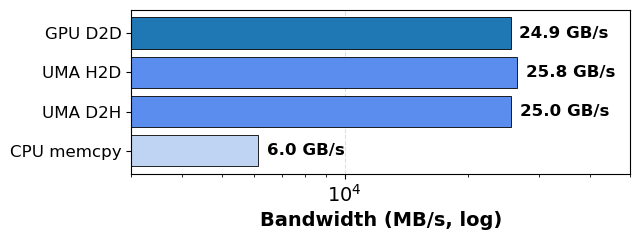
\includegraphics[width=\linewidth]{Figures/edge_back2.png}
        \caption{Unified DRAM (LPDDR5).}
        \label{fig:bg_bw_dram}
    \end{subfigure}

    \vspace{0.5em}

    \begin{subfigure}[b]{\columnwidth}
        \centering
        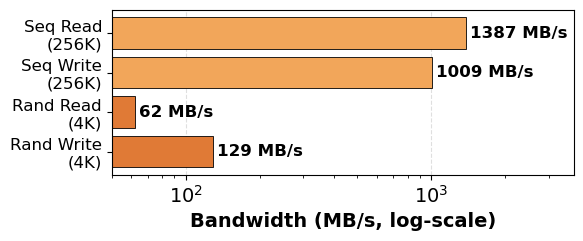
\includegraphics[width=\linewidth]{Figures/edge_back3.png}
        \caption{External NVMe SSD.}
        \label{fig:bg_bw_nvme}
    \end{subfigure}
    \vspace{-.2cm}

    \caption{Bandwidth across the edge memory hierarchy on the Jetson Orin Nano. Unified DRAM bandwidth is measured via CUDA memory copy operations. External NVMe SSD bandwidth is evaluated using FIO~\cite{} with \texttt{O\_DIRECT} (256~KB blocks for sequential and 4~KB blocks for random accesses).}
    \label{fig:bg_bandwidth}
    \vspace{-.2cm}
\end{figure}

To handle data-intensive applications such as quantum simulation on edge devices, it is necessary to understand the underlying memory architecture. Unlike HPC clusters that use discrete CPUs and GPUs connected via PCIe, edge devices such as the NVIDIA Jetson Orin Nano use a System-on-Chip (SoC) design with a Unified Memory Architecture (UMA)~\cite{nvidia2022jetson}. In this architecture, the CPU and GPU share a single physical DRAM pool, eliminating PCIe data transfers. However, this integrated design introduces bandwidth asymmetry depending on the access path and storage tier.

\noindent\textbf{Unified Memory Architecture. }
As shown in Figure~\ref{fig:bg_bw_dram}, within LPDDR5 DRAM, GPU-driven and UMA transfers (e.g., GPU D2D, UMA H2D/D2H) deliver about 25~GB/s, whereas host-driven CPU memory copies achieve only 6.0~GB/s. This is a 4$\times$ difference within the same physical memory. Recent studies in large-scale data processing propose out-of-core mechanisms~\cite{lin2022hm, hwang2020centaur} that use a user-space buffer manager to prefetch data and overlap I/O with computation. However, applying these techniques to quantum simulation on unified memory architectures presents challenges. Existing frameworks assume separate memory spaces and rely on host-driven staging. This causes their data movement to be limited by the 6.0~GB/s CPU memcpy rate, failing to exploit the higher UMA bandwidth.

\noindent\textbf{External Storage Device. }
As shown in Figure~\ref{fig:bg_bw_nvme}, when data moves to the external NVMe SSD, bandwidth decreases significantly. Sequential reads and writes provide about 1.38~GB/s and 1.0~GB/s. This is an 18$\times$ reduction compared to UMA transfers. Small-block random accesses reduce bandwidth further to 62~MB/s, which is a 400$\times$ reduction. Existing out-of-core approaches rely on operating system virtual memory management (OS-native swapping) to handle data larger than physical memory. However, the OS memory manager does not consider quantum gate access patterns, where memory stride increases exponentially with the target qubit index. Because this strided access pattern defeats standard OS readahead heuristics, page faults generate small-block storage accesses. This forces the NVMe drive into the random read state, reducing bandwidth to 62~MB/s. Consequently, this gap between the GPU kernel and OS file system leads to I/O thrashing and low GPU utilization. Furthermore, the physical storage capacity is limited to approximately 256~GB, which is insufficient to store raw state vectors of 35 qubits or more ($\geq256$~GB).

Optimizing quantum simulation on edge devices requires a specialized memory management strategy. The design must use zero-copy capabilities of UMA to sustain 25~GB/s bandwidth. It must enforce large sequential NVMe accesses (1.38~GB/s) to avoid the 62~MB/s random I/O penalty. \EdgeQuantum implements a UVM-aware asynchronous pipeline. It combines sequential I/O scheduling with zero-copy computation and maintains performance when the state vector exceeds physical memory capacity.